\documentclass[class=article, crop=false]{standalone}
\usepackage{tikz}
\usepackage{subcaption}
\usetikzlibrary{calc}
\usetikzlibrary {shapes.geometric}

\begin{document}
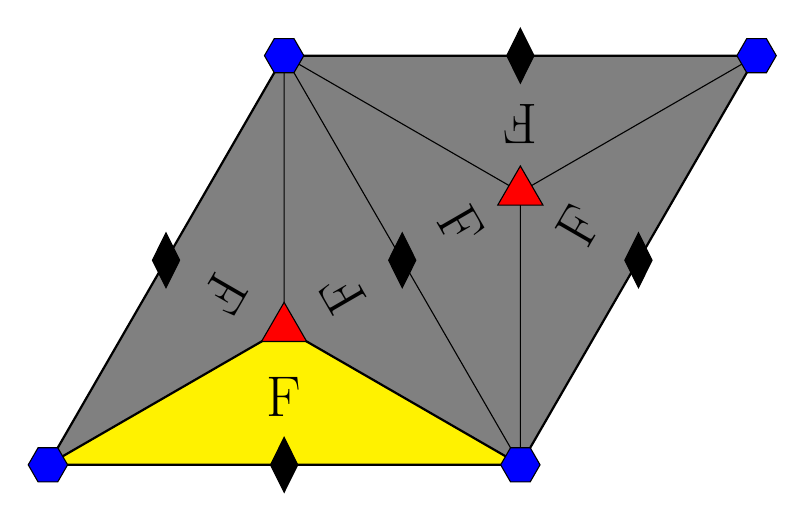
\begin{tikzpicture}
        % Define the lengths of the sides and the angle
        \def\a{3}  % length of side a
        \def\b{3}  % length of side b
        \def\angle{60}  % angle between sides a and b
        \def\s{F} % Label in center of cells
    
        % Calculate the coordinates of the points
        \coordinate (C00) at (0, 0);
        \coordinate (C10) at (\a, 0);
        \coordinate (C11) at ({\a + \b*cos(\angle)}, {\b * sin(\angle)});
        \coordinate (C01) at ({\b * cos(\angle)}, {\b * sin(\angle)});
        \coordinate (C02) at ({2*\b*cos(\angle)}, {2*\b * sin(\angle)});
        \coordinate (C12) at ({\a +2*\b * cos(\angle)}, {2*\b * sin(\angle)});
        \coordinate (C22) at ({2*\a + 2*\b * cos(\angle)}, {2*\b * sin(\angle)});
        \coordinate (C21) at ({2*\a + \b*cos(\angle)}, {\b * sin(\angle)});
        \coordinate (C20) at ({2*\a}, 0);

        \coordinate (A1) at ($(C00)!0.6666!(C11)$);
        \coordinate (A2) at ($(C11)!0.3333!(C22)$);
    
        % Draw the oblique unit cell
        \draw[thick,fill=gray] (C00) -- (C20) -- (C22) -- (C02) -- cycle;
        \draw[thick,fill=yellow] (C00) -- (A1) -- (C20) -- cycle;
        %\draw[thick] (C10) -- (C21) -- (C12) -- (C01) -- cycle;
        
        % Draw mirrow lines
        \draw[thin] (C02) -- (A1);
        \draw[thin] (C02) -- (C11) -- (C20);
        \draw[thin] (C02) -- (A2) -- (C20);
        \draw[thin] (A2) -- (C22);
        
        % Draw chiral center
        \node at ($(C00)!0.5!(C20)!0.5!(A1)$) {\huge \s};
        \node[rotate=240] at ($(C00)!0.5!(C02)!0.5!(A1)$) {\huge \s};
        \node[rotate=120] at ($(C20)!0.5!(C02)!0.5!(A1)$) {\huge \s};
        \node[rotate=300] at ($(C20)!0.5!(C02)!0.5!(A2)$) {\huge \s};
        \node[rotate=60] at ($(C22)!0.5!(C20)!0.5!(A2)$) {\huge \s};
        \node[rotate=180] at ($(C02)!0.5!(C22)!0.5!(A2)$) {\huge \s};

        % Draw node rotations
        \draw (C00)  node[regular polygon, regular polygon sides=6, draw, fill=blue, minimum size=0.5cm] {};
        \draw (C10)  node[shape aspect=0.5,diamond,draw,fill=black] {};
        \draw (C21)  node[shape aspect=0.5,diamond,draw,fill=black] {};
        \draw (C01)  node[shape aspect=0.5,diamond,draw,fill=black] {};
        \draw (C12)  node[shape aspect=0.5,diamond,draw,fill=black] {};
        \draw (C02)  node[regular polygon, regular polygon sides=6, draw, fill=blue, minimum size=0.5cm] {};
        %\draw (C12)  node[shape aspect=0.5,rotate=90,diamond,draw,fill=blue] {};
        \draw (C22)  node[regular polygon, regular polygon sides=6, draw, fill=blue, minimum size=0.5cm] {};
        %\draw (C21)  node[shape aspect=0.5,rotate=90,diamond,draw,fill=blue] {};
        \draw (C20)  node[regular polygon, regular polygon sides=6, draw, fill=blue, minimum size=0.5cm] {};

        \draw (A1)  node[regular polygon, regular polygon sides=3, draw, fill=red, minimum size=0.5cm] {};
        \draw (A2)  node[regular polygon, regular polygon sides=3, draw, fill=red, minimum size=0.5cm] {};

        \draw (C11) node[shape aspect=0.5,diamond,draw,fill=black] {};
        
    \end{tikzpicture}
\end{document}